\documentclass[11pt]{article}
\usepackage{ghb}

% On the site these become semantic block quotations styled by site.css.  The
% PDF gets a matching shaded panel rather than a plain indented quotation.
\ifdefined\ghbHTML
  \newenvironment{promptbox}{\begin{quote}}{\end{quote}}
\else
  \usepackage{tcolorbox}
  \newtcolorbox{promptbox}{
    colback=black!4,
    colframe=black!20,
    boxrule=0.4pt,
    arc=2pt,
    left=8pt,
    right=8pt,
    top=6pt,
    bottom=6pt,
    before skip=10pt,
    after skip=10pt
  }
\fi

\title{A Galactic Singularity}
\date{2026-10-21}

\summary{We're safe from $\omega$...for now}

\begin{document}

\begin{abstract}
Since the \href{https://scottaaronson.blog/?p=10169}{mathocalypse} began on 2026-10-06, it has been a strange and unsettling time.
	Amongst other things, OpenAI announced $\omega \leq \frac{9}{4}$, i.e., there exists an $O(n^{9\mathord{/}4+o(1)})$ time algorithm for matrix multiplication.
But hold on, doesn't dramatically faster matrix multiplication mean dramatically faster training of LLMs .. don't you realise $QK^T$ !?!
The singularity is here!!!

	This at least, has given me some comic relief from deciding how much to increase my $P(\mbox{doom})$ by.
\end{abstract}


\section{The Hype}

Like any sensible person, I was astounded by \href{https://github.com/openai/math}{OpenAI's mathdump}. Reality had caught up to the hype, I thought. Except I was wrong, of course, because then this hype arrived:

\begin{figure}[htbp]
  \centering
  \href{https://officechai.com/ai/openai-has-found-a-far-faster-way-to-multiply-matrices-the-math-that-underpins-all-of-modern-ai/}{%
    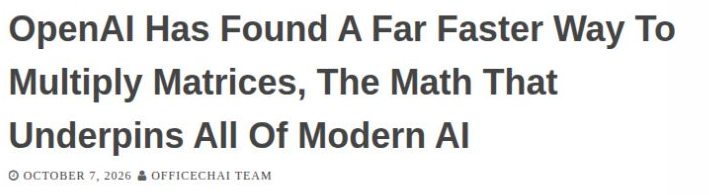
\includegraphics[width=\linewidth]{assets/galactic-singularity/officechai-headline.png}}
\end{figure}

\begin{figure}[htbp]
  \centering
  \href{https://takesonai.com/1338/the-end-of-mathematics-human-research-frontier-ai}{%
    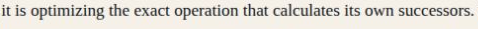
\includegraphics[width=0.80\linewidth]{assets/galactic-singularity/takesonai-successors.png}}\par\medskip
  \href{https://takesonai.com/1338/the-end-of-mathematics-human-research-frontier-ai}{%
    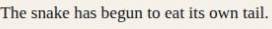
\includegraphics[width=0.46\linewidth]{assets/galactic-singularity/takesonai-snake.png}}
\end{figure}

Google's \href{https://arxiv.org/abs/2608.16884}{earlier exponent improvement} had already inspired the same enthusiasm:

\begin{figure}[htbp]
  \centering
  \href{https://news.ycombinator.com/item?id=49977146}{%
    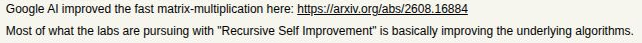
\includegraphics[width=\linewidth]{assets/galactic-singularity/hn-self-improvement.png}}
\end{figure}

I also saw this cunningly hilarious comment:

\begin{figure}[htbp]
  \centering
  \href{https://www.linkedin.com/posts/pbrzyski_the-singularity-is-going-to-be-boring-deepmind-activity-7495722525323173888-0fQO}{%
    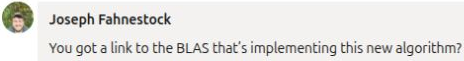
\includegraphics[width=0.80\linewidth]{assets/galactic-singularity/linkedin-blas.png}}
\end{figure}

I am no expert in fast algebraic matrix multiplication algorithms, but I had dim memories of them being \textit{\textbf{very}} impractical.

\section{It Got Weird After Strassen}

Back in the days when studying computer science was still a thing, Strassen's matrix multiplication algorithm was sometimes taught in algorithms classes. It is pretty weird when you first see it.

It lets you multiply two $n \times n$ matrices, by recursing into only \textit{seven} matrix multiplication subproblems of size $n\mathord{/}2 \times n\mathord{/}2$. This is weird because there are 8 block-multiplies to do, but
you can get away with just 7.

This results in the funny $O(n^{\log_2 7}) = O(n^{2.8073\ldots})$ time for Strassen's original matrix multiplication algorithm. Apparently, this algorithm does get some use in practice.

Now, far beyond my pay-grade, people have hammered away at getting faster algorithms. If we are \textit{very} optimistic about making these algorithms practical, they \textit{still} run into an extreme trade-off between the reduction in exponent
and the constant inside the big-Oh.

A nice example: improving Strassen's algorithm to one taking $O(n^{2.796})$ time, i.e. an exponent improvement of roughly $0.01$, increases the leading constant inside the big-Oh by a factor of about $36$.
For this to have a hope of helping in practice, we'd need $n^{0.01} > 36$, or $n > 4.3 \times 10^{155}$.

\textsc{That is a big matrix}. It would have something like $k^4$ entries, where $k$ is $\textsc{the number of atoms in the visible universe}$
(see \href{https://arxiv.org/html/2410.20538v1\#S1}{this lovely paper} for more details).
This is the realm of \href{https://en.wikipedia.org/wiki/Galactic_algorithm}{galactic algorithms}!


\section{The Final Insult, Courtesy of OpenAI}

OK, so those old-hat fast matrix multiplication algorithms are out, but now we have OpenAI's breakthrough $O(n^{2.25+\epsilon})$ time \href{https://github.com/openai/math/blob/main/preprints/Matrix-Multiplication-Nine-Fourths-October-2-2026/paper.pdf}{algorithm}. Perhaps \textit{this} algorithm is ripe
for porting to GPUs and hastening the singularity?

Well, it \href{https://www.paradigm3.org/research/mass-math\#complexity-matrix-multiplication-with-exponent-below-237}{seems} OpenAI gave an \textit{existence proof} for such an algorithm.
We have a proof that a fast algorithm exists. We don't have the recipe! This is before even worrying about what the leading constant is.

Now, maybe an AI will discover a \textit{practical} fast matrix multiplication algorithm, but this is most definitely not the one that will cause the \href{https://intelligence.org/files/AIFoomDebate.pdf}{foom}.

\begin{center}
  \rule{0.25\linewidth}{0.4pt}
\end{center}

\noindent\textbf{P.S.} Funnily enough, on the day I write this a biological intelligence calling itself Rafael Pass has given a constructive version of OpenAI's $O(n^{2.25+\epsilon})$ \href{https://arxiv.org/pdf/2610.28627}{algorithm} (sadly, he explicitly rules
out firing it up on GPUs just yet, remarking \textit{The algorithm remains ``galactic'': the constants hidden in the $O(\cdot)$ notation are enormous})

\end{document}
